\begin{ejercicio}{1}
	Determinar si es verdadero o falso, y justificar: si \( u \) y \( v \) son los únicos vértices de grado impar en un grafo, entonces \( G \) contiene un \( uv \)-camino.
\end{ejercicio}
\begin{proof}
	Notemos primero que \( u \) y \( v \) deben pertenecer a la misma componente conexa de \( G \): en cualquier componente conexa, la suma de los grados de sus vértices es par, por lo que la cantidad de vértices de grado impar dentro de ella también es par. Como \( u \) y \( v \) son los \emph{únicos} vértices de grado impar de \( G \), una componente que contenga a uno de ellos no puede tener una cantidad impar de vértices de grado impar quedando el otro afuera; luego ambos están en la misma componente \( H \) (las demás componentes, si las hay, tienen todos sus vértices de grado par).

	Trabajemos entonces dentro de \( H \). Agreguemos la arista \( uv \) a \( H \) y llamemos \( H' \) al grafo resultante. En \( H' \), todos los vértices tienen grado par y \( H' \) sigue siendo conexo, por lo que \( H' \) tiene un circuito euleriano. Este circuito euleriano debe pasar por la arista \( uv \), pero podemos mirar la parte del circuito que va de \( u \) a \( v \) sin pasar por \( uv \) o, en el otro caso, el que va de \( v \) a \( u \) sin pasar por esa arista, obteniendo así un \( uv \)-camino (que también es un \( uv \)-camino en \( G \), ya que \( H \) es subgrafo de \( G \)).
\end{proof}

\vspace{0.5cm}

\begin{ejercicioEntregar}{2}
	Probar si las siguientes son secuencias de grados de un grafo simple. En caso afirmativo, construir un grafo con esos grados. Si no, dar una prueba de imposibilidad.
	\begin{itemize}
		\item \( 5, 5, 4, 3, 2, 2, 2, 1 \)
		\item \( 5, 5, 4, 4, 2, 2, 1, 1 \)
		\item \( 5, 5, 5, 3, 2, 2, 1, 1 \)
		\item \( 5, 5, 5, 4, 2, 1, 1, 1 \)
	\end{itemize}
\end{ejercicioEntregar}
\begin{proof}
	Recordemos el \textbf{algoritmo} visto en la teoría para determinar si una secuencia de enteros no negativos \( d_1, \ldots, d_n \) es la secuencia de grados de un grafo simple. Sea \( d_1 \geq d_2 \geq \cdots \geq d_n \). Si \( d_1 = 0 \), entonces todos los \( d_i = 0 \) y la secuencia es gráfica. Si \( d_1 > 0 \), eliminamos el primer elemento \( d_1 \) y le restamos 1 a los siguientes \( d_1 \) elementos. Luego reordenamos la secuencia resultante y repetimos el proceso hasta que lleguemos a una secuencia de ceros o a una secuencia que no sea válida (por ejemplo, si algún elemento se vuelve negativo).

	Hagamos esto para cada una de las secuencias dadas:
	\begin{itemize}
		\item \textbf{Secuencia 1:} \( 5, 5, 4, 3, 2, 2, 2, 1 \)
		      \[
			      5, 5, 4, 3, 2, 2, 2, 1 \to 4, 3, 2, 1, 1, 2, 1 \to 4, 3, 2, 2, 1, 1, 1 \to 2, 1, 1, 0, 1, 1 \to 2, 1, 1, 1, 1, 0
		      \]
		      \[
			      \to 0, 0, 1, 1, 0 \to 1, 1, 0, 0, 0 \to 0, 0, 0, 0 \implies \text{Secuencia válida.}
		      \]

		\item \textbf{Secuencia 2:} \( 5, 5, 4, 4, 2, 2, 1, 1 \)
		      \[
			      5, 5, 4, 4, 2, 2, 1, 1 \to 4, 3, 3, 1, 1, 1, 1 \to 2, 2, 0, 0, 1, 1 \to 2, 2, 1, 1, 0, 0
		      \]
		      \[
			      \to 1, 0, 1, 0, 0 \to 1, 1, 0, 0, 0 \to 0, 0, 0, 0 \implies \text{Secuencia válida.}
		      \]

		\item \textbf{Secuencia 3:} \( 5, 5, 5, 3, 2, 2, 1, 1 \)
		      \[
			      5, 5, 5, 3, 2, 2, 1, 1 \to 4, 4, 2, 1, 1, 1, 1 \to 3, 1, 0, 0, 1, 1 \to 3, 1, 1, 1, 0, 0
		      \]
		      \[
			      \to 0, 0, 0, 0, 0 \implies \text{Secuencia válida.}
		      \]

		\item \textbf{Secuencia 4:} \( 5, 5, 5, 4, 2, 1, 1, 1 \)
		      \[
			      5, 5, 5, 4, 2, 1, 1, 1 \to 4, 4, 3, 1, 0, 1, 1 \to 4, 4, 3, 1, 1, 1, 0 \to 3, 2, 0, 0, 1, 0
		      \]
		      \[
			      \to 3, 2, 1, 0, 0, 0 \to 1, 0, -1, 0, 0 \implies \text{Secuencia \textbf{NO} válida, aparece un grado negativo}
		      \]
	\end{itemize}

	\vspace{0.5cm}
	A continuación, construimos los grafos simples correspondientes para las secuencias válidas. Nombramos los vértices \(v_1, \ldots, v_8\) donde el subíndice respeta el orden original de la secuencia de mayor a menor grado.

	\begin{center}
		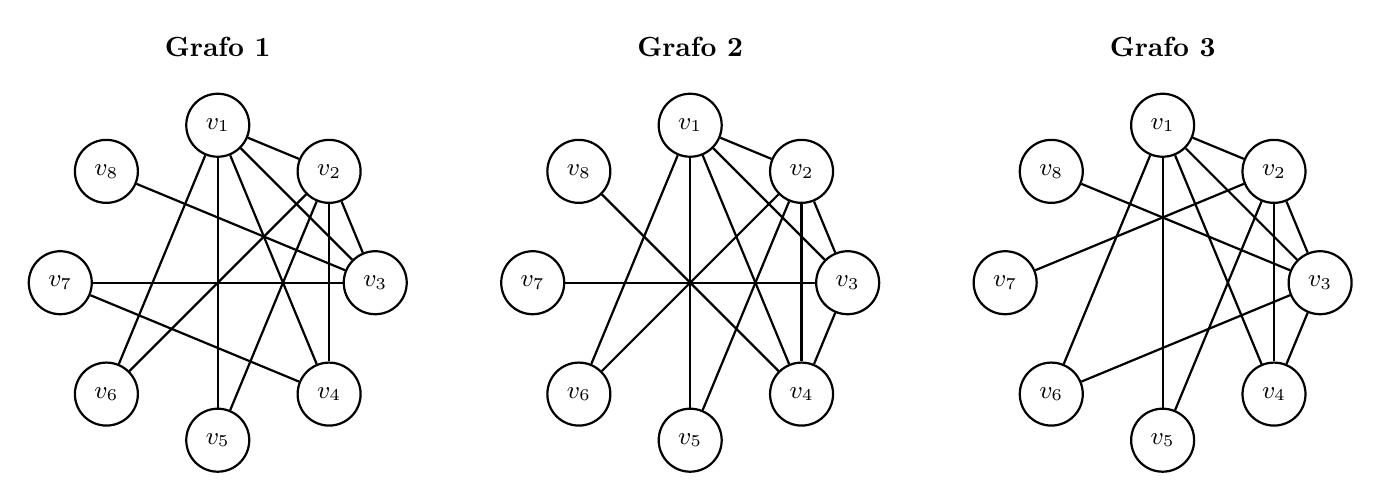
\begin{tikzpicture}[
				vertex/.style={circle, draw, minimum size=8mm, inner sep=0pt, font=\small},
				thick]

			\node at (0, 3) {\textbf{Grafo 1}};
			% Grafo 1: 5, 5, 4, 3, 2, 2, 2, 1
			\begin{scope}[shift={(0,0)}]
				\foreach \i/\ang in {1/90, 2/45, 3/0, 4/-45, 5/-90, 6/-135, 7/-180, 8/135} {
						\node[vertex] (g1v\i) at (\ang:2) {$v_{\i}$};
					}
				% Aristas Grafo 1
				\draw (g1v1) -- (g1v2); \draw (g1v1) -- (g1v3); \draw (g1v1) -- (g1v4); \draw (g1v1) -- (g1v5); \draw (g1v1) -- (g1v6);
				\draw (g1v2) -- (g1v3); \draw (g1v2) -- (g1v4); \draw (g1v2) -- (g1v5); \draw (g1v2) -- (g1v6);
				\draw (g1v3) -- (g1v7); \draw (g1v3) -- (g1v8);
				\draw (g1v4) -- (g1v7);
			\end{scope}

			\node at (6, 3) {\textbf{Grafo 2}};
			% Grafo 2: 5, 5, 4, 4, 2, 2, 1, 1
			\begin{scope}[shift={(6,0)}]
				\foreach \i/\ang in {1/90, 2/45, 3/0, 4/-45, 5/-90, 6/-135, 7/-180, 8/135} {
						\node[vertex] (g2v\i) at (\ang:2) {$v_{\i}$};
					}
				% Aristas Grafo 2
				\draw (g2v1) -- (g2v2); \draw (g2v1) -- (g2v3); \draw (g2v1) -- (g2v4); \draw (g2v1) -- (g2v5); \draw (g2v1) -- (g2v6);
				\draw (g2v2) -- (g2v3); \draw (g2v2) -- (g2v4); \draw (g2v2) -- (g2v5); \draw (g2v2) -- (g2v6);
				\draw (g2v3) -- (g2v4); \draw (g2v3) -- (g2v7);
				\draw (g2v4) -- (g2v8);
			\end{scope}

			\node at (12, 3) {\textbf{Grafo 3}};
			% Grafo 3: 5, 5, 5, 3, 2, 2, 1, 1
			\begin{scope}[shift={(12,0)}]
				\foreach \i/\ang in {1/90, 2/45, 3/0, 4/-45, 5/-90, 6/-135, 7/-180, 8/135} {
						\node[vertex] (g3v\i) at (\ang:2) {$v_{\i}$};
					}
				% Aristas Grafo 3
				\draw (g3v1) -- (g3v2); \draw (g3v1) -- (g3v3); \draw (g3v1) -- (g3v4); \draw (g3v1) -- (g3v5); \draw (g3v1) -- (g3v6);
				\draw (g3v2) -- (g3v3); \draw (g3v2) -- (g3v4); \draw (g3v2) -- (g3v5); \draw (g3v2) -- (g3v7);
				\draw (g3v3) -- (g3v4); \draw (g3v3) -- (g3v6); \draw (g3v3) -- (g3v8);
			\end{scope}
		\end{tikzpicture}
	\end{center}
\end{proof}

\vspace{0.5cm}

\begin{ejercicio}{3}
	Se tiene una liga con dos divisiones de 13 equipos cada una. Determinar si es posible programar la temporada de manera que cada equipo juegue nueve partidos con equipos de su división y cuatro partidos con equipos de la otra división.
\end{ejercicio}
\begin{proof}
	Si separamos cada división y vemos los partidos que se juegan dentro de cada división, tenemos que cada equipo juega 9 partidos con equipos de su división. Esto quiere decir que, si pensamos cada equipo como un vértice, tenemos que armar el grafo con la siguiente secuencia de números: \[
		9, 9, 9, 9, 9, 9, 9, 9, 9, 9, 9, 9, 9
	\]
	Cuya suma total es \( 9 \cdot 13 = 117 \), que es impar. Por lo tanto, no es posible que los equipos jueguen 9 partidos con equipos de su división y, por lo tanto, no es posible programar la temporada de la manera que se pide.
\end{proof}

\vspace{0.5cm}

\begin{ejercicioEntregar}{4}
	Probar que todo grafo simple con al menos dos vértices tiene dos vértices de igual grado ¿Vale lo mismo para grafos sin loops con aristas múltiples?
\end{ejercicioEntregar}
\begin{proof}
	Sea \( G \) un grafo simple con \( n \geq 2 \) vértices. Los posibles grados de los vértices en un grafo simple con \( n \) vértices son \( 0, 1, 2, \ldots, n-1 \). Esto nos da \( n \) posibles grados. Supongamos que los \( n \) vértices tienen todos grados distintos. Si aplicamos el algoritmo, nos queda:\[
		n-1, n-2, n-3, \ldots, 2, 1, 0 \to n-3, n-4, \ldots, 1, -1
	\]
	Luego, no es posible armar un grafo de estas características.

	No vale lo mismo para grafos sin loops con aristas múltiples. Por ejemplo, el grafo de 3 vértices con una simple y una arista múltiple entre dos de ellos tiene grados \( 1, 2, 3 \) y no hay dos vértices con el mismo grado.
\end{proof}

\vspace{0.5cm}

\begin{ejercicio}{5}
	Sean \( d_1, \ldots, d_n \) enteros tales que \( d_1 \geq \cdots \geq d_n \geq 0 \). Probar que existe un grafo sin loops (se permiten aristas múltiples) con secuencia de grados \( d_1, \ldots, d_n \) si y sólo si la suma de estos números es par y \( d_1 \leq d_2 + \cdots + d_n \).
\end{ejercicio}
\begin{proof}
	Sean \( d_1, \ldots, d_n \) enteros tales que \( d_1 \geq \cdots \geq d_n \geq 0 \).
	\begin{itemize}
		\item[\(\Longrightarrow\))] Supongamos que existe un grafo \( G \) sin loops con secuencia de grados \( d_1, \ldots, d_n \). La suma de los grados siempre es par. Luego,
		      \[
			      \sum_{i=1}^n d_i = 2 |E(G)|
		      \]
		      Como no hay loops, el grado de cualquier vértice a lo sumo puede ser igual a la cantidad total de aristas en el grafo, por lo que \( d_1 \le |E(G)| \). Sustituyendo esto, tenemos:
		      \[
			      d_1 \le \sum_{i=1}^n \frac{d_i}{2} \implies 2d_1 \le \sum_{i=1}^n d_i \implies 2d_1 \le d_1 + \sum_{i=2}^n d_i \implies d_1 \le d_2 + \cdots + d_n
		      \]

		\item[\(\Longleftarrow\))] Sea \( d_1 \le d_2 + \cdots + d_n \) y supongamos que \( \sum_{i=1}^n d_i \) es par.
		      Llamemos \( S = \sum_{i=1}^n d_i \). Como \( S \) es par, podemos escribir \( S = 2m \).
		      Por hipótesis, \( d_1 \le \sum_{i=2}^n d_i \). Sumando \( d_1 \) a ambos lados obtenemos \( 2d_1 \le S = 2m \), lo que implica que \( d_1 \le m \).

		      Vamos a construir un grafo \( G \). Consideremos un conjunto de \( 2m \) puntos, numerados del \( 1 \) al \( 2m \).
		      Asignamos estos puntos a los vértices de manera secuencial en bloques contiguos:
		      \begin{itemize}
			      \item Al vértice \( v_1 \) le asignamos los primeros \( d_1 \) puntos.
			      \item Al vértice \( v_2 \) le asignamos los siguientes \( d_2 \) puntos.
			      \item Y así sucesivamente; en general, a cada vértice \( v_i \) le asignamos un bloque de \( d_i \) puntos.
		      \end{itemize}

		      Para formar las aristas de \( G \), unimos el punto \( j \) con el punto \( j+m \) para todo \( 1 \le j \le m \).

		      Es evidente que cada vértice \( v_i \) tendrá grado exactamente \( d_i \), puesto que le asignamos \( d_i \) puntos y cada punto forma exactamente un extremo de una arista.

		      Resta verificar que el grafo resultante no tiene loops. Un loop se formaría si conectamos el punto \( j \) con el punto \( j+m \) y ambos pertenecen al mismo vértice \( v_i \). Sin embargo, la cantidad de puntos asignados al vértice \( v_i \) es \( d_i \). Como la secuencia está ordenada de forma decreciente, el vértice con más puntos es \( v_1 \), el cual tiene \( d_1 \) puntos.
		      Dado que \( d_1 \le m \), la distancia máxima entre los números de dos puntos que pertenecen al mismo vértice es estrictamente menor que \( m \).
		      Por lo tanto, el punto \( j \) y el punto \( j+m \) nunca pueden pertenecer al mismo vértice. Esto garantiza que no se forman loops, concluyendo la demostración.
	\end{itemize}
\end{proof}

\vspace{0.5cm}

\begin{ejercicio}{6}
	Determinar si es verdadero o falso y justificar: todo digrafo simple (permitiendo loops) con \( n \) vértices (\( n > 1 \)) tiene dos vértices distintos con el mismo grado de salida o dos vértices distintos con el mismo grado de llegada ¿Cambia la respuesta si pensamos a los digrafos simples en el sentido más restrictivo de que los loops no están permitidos?
\end{ejercicio}
\begin{proof}
	\emph{Claim}: La afirmación es \textbf{falsa} en ambos casos.

	\begin{center}
		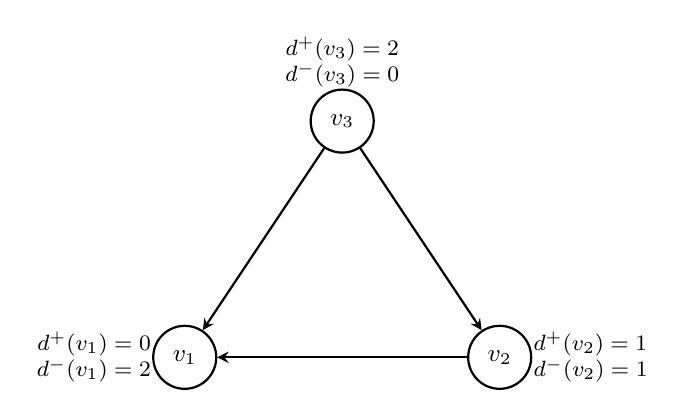
\begin{tikzpicture}[
				vertex/.style={circle, draw, minimum size=8mm, inner sep=0pt, font=\small}, ->, >=stealth, thick]

			\node[vertex] (v1) at (0, 0) {$v_1$};
			\node[vertex] (v2) at (4, 0) {$v_2$};
			\node[vertex] (v3) at (2, 3) {$v_3$};

			\draw (v3) -- (v2);
			\draw (v3) -- (v1);
			\draw (v2) -- (v1);

			% Etiquetas de grados
			\node[align=left, font=\footnotesize, right=0.3cm] at (v2) {$d^+(v_2)=1$\\$d^-(v_2)=1$};
			\node[align=right, font=\footnotesize, left=0.3cm] at (v1) {$d^+(v_1)=0$\\$d^-(v_1)=2$};
			\node[align=center, font=\footnotesize, above=0.3cm] at (v3) {$d^+(v_3)=2$\\$d^-(v_3)=0$};

		\end{tikzpicture}
	\end{center}

	Los grados de salida son \( d^+(v_1)=0 \), \( d^+(v_2)=1 \), \( d^+(v_3)=2 \) (todos distintos).
	Los grados de llegada son \( d^-(v_1)=2 \), \( d^-(v_2)=1 \), \( d^-(v_3)=0 \) (todos distintos).

	Como el grafo no utiliza loops, los grados de salida y llegada siguen siendo distintos para cada vértice. Por lo tanto, la afirmación es falsa en ambos casos.
\end{proof}

\vspace{0.5cm}

\begin{definition}
	Un \textbf{camino dirigido} en un digrafo \( D \) es una secuencia de vértices \( v_1, v_2, \ldots, v_k \) tal que para cada \( i = 1, 2, \ldots, k-1 \), existe una arista dirigida de \( v_i \) a \( v_{i+1} \).
\end{definition}

\begin{definition}
	Un digrafo se dice \textbf{fuertemente conexo} si para cada par de vértices \( u \) y \( v \), existe un camino dirigido de \( u \) a \( v \) y otro de \( v \) a \( u \).
\end{definition}

\begin{ejercicioEntregar}{7}
	Dos vértices de un digrafo \( x \) e \( y \) se dicen conectados si existe un camino dirigido de \( x \) a \( y \) y otro de \( y \) a \( x \). Probar que la relación de conexión en un digrafo \( D \) es de equivalencia y que sus clases son las componentes fuertemente conexas de \( D \).
\end{ejercicioEntregar}
\begin{proof}
	Para ver que es una relación de equivalencia, debemos verificar que es reflexiva, simétrica y transitiva. Llamemos \( \sim \) a esta relación de conexión, es decir, \( x \sim y \) si y sólo si existe un camino dirigido de \( x \) a \( y \) y otro de \( y \) a \( x \).

	\begin{itemize}
		\item \textbf{Reflexiva (\( x \sim x \)):} Para cualquier vértice \( x \in V(D) \), la secuencia formada por el único vértice \( x \) constituye un camino dirigido de longitud 0 (camino trivial o vacío) de \( x \) a \( x \). Por lo tanto, \( x \sim x \).

		\item \textbf{Simétrica (\( x \sim y \implies y \sim x \)):} Si \( x \sim y \), entonces por definición existe un camino dirigido de \( x \) a \( y \) y otro de \( y \) a \( x \). Esto es equivalente a decir que existe un camino de \( y \) a \( x \) y otro de \( x \) a \( y \), por lo que \( y \sim x \).

		\item \textbf{Transitiva (\( x \sim y \) e \( y \sim z \implies x \sim z \)):} Si \( x \sim y \), existen caminos dirigidos \( P_{xy} \) (de \( x \) a \( y \)) y \( P_{yx} \) (de \( y \) a \( x \)). Como \( y \sim z \), existen caminos dirigidos \( P_{yz} \) y \( P_{zy} \). Concatenando \( P_{xy} \) con \( P_{yz} \) obtenemos un recorrido dirigido de \( x \) a \( z \), del cual siempre podemos extraer un camino dirigido de \( x \) a \( z \). Análogamente, concatenando \( P_{zy} \) con \( P_{yx} \) obtenemos un recorrido del cual extraemos un camino dirigido de \( z \) a \( x \). Por lo tanto, \( x \sim z \).
	\end{itemize}

	Luego, la relación de conexión \( \sim \) es de equivalencia.

	Veamos ahora que las clases de equivalencia bajo esta relación son precisamente las componentes fuertemente conexas del digrafo \( D \).

	Por un lado, la clase de equivalencia de un vértice \( x \), denotada \( [x] \), es el conjunto de todos los vértices \( y \) tales que \( x \sim y \). Por definición de \( \sim \), todos los vértices en \( [x] \) son mutuamente alcanzables, formando un conjunto fuertemente conexo.

	Además, las clases de equivalencia son subconjuntos \textbf{maximales} respecto a esta propiedad: si existiera un vértice \( w \notin [x] \) que fuera mutuamente alcanzable con los vértices de \( [x] \), en particular tendríamos \( x \sim w \), lo que implicaría \( w \in [x] \), llegando a un absurdo.

	Dado que una componente fuertemente conexa se define justamente como un subgrafo fuertemente conexo maximal, concluimos que las clases de equivalencia de \( \sim \) coinciden exactamente con las componentes fuertemente conexas de \( D \).
\end{proof}

\vspace{0.5cm}

\begin{ejercicioEntregar}{8}
	Probar que en todo digrafo existe una componente fuertemente conexa sin aristas que ingresen a ella y que existe una componente fuertemente conexa sin aristas que salgan de ella.
\end{ejercicioEntregar}
\begin{proof}
	Sea \( D \) un digrafo (asumimos finito) y consideremos su grafo de componentes fuertemente conexas, \( D^* \). En \( D^* \), cada vértice representa una componente fuertemente conexa de \( D \), y hay una arista dirigida de la componente \( C_i \) a la componente \( C_j \) si existe al menos una arista en \( D \) desde algún vértice en \( C_i \) hacia algún vértice en \( C_j \).

	Si el grafo \( D^* \) tuviera un ciclo dirigido, esto implicaría que todos los vértices de las componentes involucradas en el ciclo serían mutuamente alcanzables en \( D \). Pero entonces todas ellas formarían una única gran componente fuertemente conexa, lo que contradice la definición de las componentes originales. Por lo tanto, \( D^* \) es un digrafo acíclico.

	Como \( D \) es finito, \( D^* \) también lo es. Veamos que en todo digrafo acíclico finito existe al menos un vértice sin aristas entrantes y al menos uno sin aristas salientes.

	Consideremos un camino dirigido de longitud máxima en \( D^* \), digamos \( P = C_1, C_2, \ldots, C_k \).
	\begin{itemize}
		\item El vértice inicial \( C_1 \) no puede tener aristas que ingresen a él. Si recibiera una arista de algún \( C_i \) perteneciente a \( P \), se formaría un ciclo (absurdo). Si recibiera una arista de un vértice externo a \( P \), el camino podría extenderse hacia atrás, contradiciendo que \( P \) es de longitud máxima. Por lo tanto, \( C_1 \) es la componente buscada sin aristas entrantes.
		\item Por un razonamiento análogo, el vértice final \( C_k \) no puede tener aristas que salgan de él (de lo contrario se formaría un ciclo o el camino se extendería hacia adelante). Luego, \( C_k \) es la componente buscada sin aristas salientes.
	\end{itemize}

	Esto demuestra la existencia de ambas componentes en el digrafo original \( D \).
\end{proof}

\vspace{0.5cm}

\begin{ejercicio}{9}
	Sea \( G \) un digrafo simple con \( n \) vértices y sin ciclos dirigidos. Probar que existe un orden \( v_1, \ldots, v_n \) de los vértices de \( G \) de modo que, para todo par de valores distintos \( i, j \) entre \( 1 \) y \( n \), si \( v_i v_j \in E(G) \) entonces \( i \leq j \).
\end{ejercicio}
\begin{proof}
	Procedemos por inducción sobre \( n \), la cantidad de vértices de \( G \).

	\paragraph{Caso base:} Si \( n = 1 \), \( G \) tiene un único vértice \( v_1 \) y ninguna arista. El orden \( v_1 \) satisface la condición trivialmente.

	\paragraph{Paso inductivo:} Supongamos que la afirmación es cierta para todo digrafo simple sin ciclos dirigidos de \( n-1 \) vértices (\( n \ge 2 \)).

	Sea \( G \) un digrafo simple sin ciclos dirigidos de \( n \) vértices. Sea \( S \) el conjunto de los vértices de \( G \) con grado de entrada igual a cero.

	Primero, demostremos que \( S \neq \varnothing \). Supongamos por el absurdo que \( S = \varnothing \implies \) todo vértice de \( G \) tiene al menos una arista entrante. Si partimos de un vértice cualquiera y retrocedemos por las aristas entrantes, podemos construir un camino infinito. Dado que \( G \) tiene una cantidad finita de vértices, en algún momento deberemos visitar un vértice por segunda vez. Esto forma un ciclo dirigido, pero \( G \) es acíclico \( \implies S \neq \varnothing \).

	Tomemos \( v \in S \) y lo fijamos como el primer elemento de la secuencia, \( v_1 = v \). Consideremos el subgrafo inducido \( G' = G - \{v_1\} \). Es claro que \( G' \) es un digrafo simple sin ciclos dirigidos y tiene \( n-1 \) vértices.

	Por \textbf{H.I}, existe un orden \( v_2, \ldots, v_n \) de los vértices de \( G' \) tal que para todo par de índices \( i, j \in \{2, \ldots, n\} \), si \( v_i v_j \in E(G') \), entonces \( i \le j \).

	Para finalizar, comprobemos que el orden \( v_1, v_2, \ldots, v_n \) es válido para la totalidad de \( G \). Tomemos una arista cualquiera \( v_i v_j \in E(G) \) y evaluemos los casos posibles:

	\begin{itemize}
		\item \textbf{Si \( i, j \ge 2 \):} estamos en la \textbf{H.I} y vale.
		\item \textbf{Si \( i = 1 \):} La arista es de la forma \( v_1 v_j \). Como \( j \in \{2, \ldots, n\} \implies 1 < j \implies i \le j \).
		\item \textbf{Si \( j = 1 \):} No existen aristas de la forma \( v_i v_1 \) pues \( v_1 \in S \).
	\end{itemize}

	En todos los casos posibles, \( v_i v_j \in E(G) \implies i \le j \). Esto completa la demostración.
\end{proof}

\vspace{0.5cm}

\begin{definition}
	Un \textbf{torneo} es un digrafo cuyo grafo subyacente es un grafo completo. En otras palabras, el digrafo obtenido de un grafo completo al darle orientación a sus aristas.
\end{definition}

\begin{ejercicio}{10}
	Probar que existe un torneo de \( n \) vértices con grado de salida igual al grado de llegada en cada vértice si y sólo si \( n \) es impar.
\end{ejercicio}
\begin{proof}
	\(\Longrightarrow\)) Sea \( G \) un torneo de \( n \) vértices tal que en cada vértice el grado de salida es igual al grado de llegada. En cualquier torneo, \(\forall v \in V(G) \) vale que \( d^+(v) + d^-(v) = n-1 \). Como por hipótesis \( d^+(v) = d^-(v) \), obtenemos \( 2d^+(v) = n-1 \implies n \) es impar.

	\(\Longleftarrow)\) Supongamos que \( n \) es impar. Queremos construir un torneo de \( n \) vértices tal que \( d^+(v) = d^-(v) \quad \forall v \in V(G) \). Sea \( k = \frac{n-1}{2} \in \N \).

	Sea el conjunto de vértices \( V = \{0, 1, \ldots, n-1\} \). Trazamos una arista dirigida de \( i \) a \( j \iff (j - i) \pmod n \in \{1, 2, \ldots, k\} \).

	Veamos que esto define un torneo. Dados dos vértices distintos \( i, j \in V \), como \( i \not\equiv j \pmod n \), ambos restos \( (j-i) \bmod n \) y \( (i-j) \bmod n \) son no nulos y pertenecen a \( \{1, \ldots, n-1\} \); además, al ser uno el opuesto del otro módulo \( n \), su suma es exactamente \( n \). Si ambos fueran \( \le k \), la suma sería a lo sumo \( 2k < n \); si ambos fueran \( \ge k+1 \), la suma sería al menos \( 2k+2 > n \). Luego, exactamente uno de los dos restos es \( \le k \), es decir, se traza exactamente una arista dirigida entre cada par de vértices, cumpliendo la definición de torneo.

	Finalmente, por construcción, para cada vértice \( i \) hay exactamente \( k \) valores distintos de \( j \) hacia los que apunta. Por lo tanto, el grado de salida de todo vértice es \( k = \frac{n-1}{2} \). Como cada vértice está conectado a \( n-1 \) vértices en total, su grado de entrada también es \( n - 1 - k = k \), cumpliéndose así lo requerido.
\end{proof}

\vspace{0.5cm}

\begin{definition}
	Un \textbf{camino dirigido hamiltoniano} en un digrafo \( D \) es un camino dirigido que visita cada vértice de \( D \) exactamente una vez.
\end{definition}

\begin{ejercicioEntregar}{11}
	Probar que todo torneo posee un camino dirigido hamiltoniano.
\end{ejercicioEntregar}
\begin{proof}
	Sea \( G \) un torneo con \( n \) vértices. Procedemos por inducción sobre \( n \).

	\paragraph{Caso base:} Si \( n = 1 \), el único vértice forma un camino hamiltoniano trivial.

	\paragraph{Paso inductivo:} Supongamos que vale para todo torneo con \( n-1 \) vértices. Sea \( G \) un torneo con \( n \) vértices. Tomemos un vértice \( v \in V(G) \) y consideremos el subgrafo inducido \( G' = G - \{v\} \), que es un torneo de \( n-1 \) vértices. Por \textbf{H.I}, existe un camino dirigido hamiltoniano en \( G' \), digamos \( P = v_1, v_2, \ldots, v_{n-1} \).

	Para extender este camino a todo \( G \), debemos insertar el vértice \( v \). Como \( G \) es un torneo, entre \( v \) y cualquier \( v_k \) existe exactamente una arista dirigida. Analizamos tres casos posibles para la inserción:

	\begin{itemize}
		\item Si \( v v_1 \in E(G) \), entonces el camino \( v, v_1, v_2, \ldots, v_{n-1} \) es un camino dirigido hamiltoniano en \( G \).

		\item Si \( v_{n-1} v \in E(G) \), entonces el camino \( v_1, v_2, \ldots, v_{n-1}, v \) es un camino dirigido hamiltoniano en \( G \).

		\item Veamos qué ocurre si \( v v_1 \notin E(G) \) y \( v_{n-1} v \notin E(G) \). Sea \( i \) el \textit{máximo} índice en el conjunto \( \{1, \ldots, n-1\} \) tal que \( v_i v \in E(G) \).
		      Sabemos que \( i \) existe y es al menos \( 1 \) (pues \( v_1 v \in E(G) \)), y sabemos que \( i < n-1 \) (pues \( v_{n-1} v \notin E(G) \)).

		      Consideremos el vértice siguiente en el camino, \( v_{i+1} \). Como \( i \) es el máximo índice que apunta a \( v \), la arista entre \( v_{i+1} \) y \( v \) no puede estar dirigida hacia \( v \). Por ser \( G \) un torneo, necesariamente sale de \( v \), es decir, \( v v_{i+1} \in E(G) \).

		      De esta manera podemos insertar \( v \) justo entre ellos, formando el camino dirigido hamiltoniano \( v_1, \ldots, v_i, v, v_{i+1}, \ldots, v_{n-1} \).
	\end{itemize}

	En todos los casos es posible construir el camino hamiltoniano, lo que completa la demostración.
\end{proof}

\vspace{0.5cm}

\begin{definition}
	Un \textbf{ciclo dirigido hamiltoniano} en un digrafo \( D \) es un ciclo dirigido que visita cada vértice de \( D \) exactamente una vez.
\end{definition}

\begin{ejercicio}{12}
	Probar que un torneo posee un ciclo hamiltoniano si y sólo si es fuertemente conexo.
\end{ejercicio}
\begin{proof}
	(\(\Longrightarrow\)) Sea \( G \) un torneo con un ciclo hamiltoniano. Sea \( C = v_1, v_2, \ldots, v_n, v_1 \) dicho ciclo. Para cualquier par de vértices \( v_i, v_j \), podemos ir de \( v_i \) a \( v_j \) siguiendo el ciclo en la dirección adecuada. Por lo tanto, existe un camino dirigido de \( v_i \) a \( v_j \) y otro de \( v_j \) a \( v_i \), lo que implica que \( G \) es fuertemente conexo.

	(\(\Longleftarrow\)) Sea \( G \) un torneo fuertemente conexo. Demostraremos que contiene un ciclo hamiltoniano tomando un ciclo de longitud máxima y probando por el absurdo que debe incluir a todos los vértices.

	Como \( G \) es fuertemente conexo (y \( n \ge 3 \), ya que para \( n=1 \) es trivial y \( n=2 \) no puede ser fuertemente conexo), cada vértice tiene grado de entrada y salida mayor a cero, lo que garantiza la existencia de al menos un ciclo.
	Sea \( C = v_1, v_2, \ldots, v_k, v_1 \) un ciclo dirigido de longitud máxima \( k \). Supongamos por el absurdo que \( k < n \).

	Sea \( W = V(G) \setminus V( C ) \) el conjunto de vértices que no están en el ciclo. Evaluamos las conexiones entre \( W \) y \( C \). Existen dos posibilidades para un vértice \( u \in W \):

	\paragraph{Caso 1:} \( u \) tiene al menos una arista hacia \( C \) y al menos una arista recibida desde \( C \).
	Por un razonamiento anáogo al ejercicio anterior, al recorrer los vértices de \( C \) en orden, la dirección de las aristas entre \( C \) y \( u \) debe cambiar en algún momento de salir de \( C \) a entrar a \( C \). Es decir, existe un índice \( i \) tal que \( v_i u \in E(G) \) y \( u v_{i+1} \in E(G) \).
	Si insertamos \( u \), formamos el ciclo \( v_1, \ldots, v_i, u, v_{i+1}, \ldots, v_k, v_1 \) de longitud \( k+1 \), lo que contradice que \( C \) era de longitud máxima.

	\paragraph{Caso 2:} Ningún vértice de \( W \) cumple el Caso 1.
	Entonces, \( W \) se divide estrictamente en dos subconjuntos: \( W_{in} \), formado por los vértices que \textit{sólo} reciben aristas desde \( C \) (y por lo tanto no envían ninguna arista hacia \( C \)); y \( W_{out} \), formado por los vértices que \textit{sólo} envían aristas hacia \( C \) (y por lo tanto no reciben ninguna arista desde \( C \)).

	Veamos primero que ambos subconjuntos son no vacíos. Si \( W_{out} = \varnothing \), entonces todo vértice de \( W \) pertenece a \( W_{in} \), y por definición ninguno de ellos envía una arista hacia \( C \); como tampoco hay otra forma de salir de \( W \) (las únicas aristas entre \( C \) y \( W \) son las que van de \( C \) a \( W_{in} \)), ningún vértice de \( W \) podría alcanzar jamás a un vértice de \( C \), contradiciendo que \( G \) es fuertemente conexo (recordar que \( W \neq \varnothing \) pues \( k < n \)). Por lo tanto \( W_{out} \neq \varnothing \). Simétricamente, si \( W_{in} = \varnothing \), entonces todo vértice de \( W \) pertenece a \( W_{out} \) y ninguno recibe una arista desde \( C \), por lo que ningún vértice de \( C \) podría alcanzar a un vértice de \( W \), contradiciendo nuevamente que \( G \) es fuertemente conexo. Luego \( W_{in} \neq \varnothing \).

	Afirmamos ahora que existe al menos un par \( y \in W_{in} \), \( x \in W_{out} \) con \( yx \in E(G) \). En efecto, supongamos por el absurdo que para todo \( y \in W_{in} \) y todo \( x \in W_{out} \) la arista va en el sentido \( xy \) (esto cubre todos los casos, pues \( G \) es un torneo y entre \( y \) y \( x \) hay exactamente una arista dirigida). Entonces ningún vértice de \( W_{in} \) tiene aristas salientes hacia \( C \) (por definición de \( W_{in} \)) ni hacia \( W_{out} \) (por la suposición), de modo que sus únicas aristas salientes posibles quedan dentro del propio \( W_{in} \). Esto implica que ningún vértice de \( W_{in} \) puede alcanzar jamás a un vértice de \( C \), contradiciendo que \( G \) es fuertemente conexo. Luego existen \( y \in W_{in} \) y \( x \in W_{out} \) con \( yx \in E(G) \).

	Pero en este escenario, sabiendo que \( v_1 \) apunta a \( y \) (pues \( y \in W_{in} \)) y que \( x \) apunta a \( v_2 \) (pues \( x \in W_{out} \)), podemos formar el ciclo \( v_1, y, x, v_2, v_3, \ldots, v_k, v_1 \). Este nuevo ciclo tiene longitud \( k+2 \), lo que vuelve a contradecir la maximidad de \( C \).

	En ambos casos llegamos a un absurdo producto de suponer que \( k < n \). Por lo tanto, \( k = n \) y el ciclo máximo \( C \) es un ciclo hamiltoniano.
\end{proof}
